\chapter{Resultados}
\label{chap:resultados}

\drop{D}{urante} el desarrollo de este capítulo se mostrarán los resultados obtenidos al seguir la planificación haciendo uso de lo detallado en el capítulo anterior, por lo que el avance se dividirá en Sprints. Cada uno de ellos tendrá, al menos, una historia de usuario asignada que estará implementada al final del desarrollo.

Debido a que el equipo de Scrum es reducido, se han tenido que realizar diversos ajustes para adoptar esta metodología al trabajo que se va a desarrollar. Por tanto, el equipo identificado queda de la siguiente manera:

\begin{itemize}
	\item \textbf{Dueño del Producto:} Luis Rodríguez Benítez.
	\item \textbf{Maestro de Scrum:} Luis Jiménez Linares.
	\item \textbf{Equipo de Scrum:} Diego Andérica Richard.
\end{itemize}

Este capítulo constará de los diferentes Sprints en los que se ha dividido el proyecto, así como su planificación y correspondientes resultados de la realización de las tareas. Antes de comenzar con el primer Sprint se ha de tener en cuenta uno de los artefactos más importantes de la metodología escogida como es la Pila de Producto, puesto que es un elemento fundamental en la metodología de Scrum ya que es donde se reflejan todas las características y requisitos que debe poseer la aplicación final, siendo elaborada en el Sprint 0 con la ayuda del dueño del producto.

\clearpage

\section{Planificación inicial (Sprint 0)}
Durante este primer Sprint se realizan tareas de vital importancia como fijar qué elementos debe poseer la solución final (Pila de Producto), el coste de llevar a cabo el proyecto o la planificación de este. También se debe realizar una tarea de estudio e investigación acerca de la arquitectura que se tiene pensado utilizar junto con las diferentes alternativas que pueden existir actualmente. Para construir la Pila de Producto se realizan diversas reuniones con el dueño del producto, con el fin de establecer las diferentes historias de usuario y las tareas que deberán abordarse para completar cada una de ellas.

\subsection{Pila de Producto}
La Pila de Producto, como se ha explicado con anterioridad, se trata de una lista de todo lo que puede ser necesario en el producto. Durante las reuniones que se han producido antes de comenzar el proyecto, el equipo de Scrum ha fijado las historias de usuario, así como su duración estimada y la prioridad para cada una. En este caso, la Pila de Producto es la que se muestra en la Tabla \ref{tab:pilaproducto}:

\begin{table}[!htbp]
	\centering
	{\small
		\begin{tabular}{|l|l|l|l|}
	\hline
	\multicolumn{4}{|c|}{\cellcolor[HTML]{343434}{\color[HTML]{FFFFFF} \textbf{Pila de Producto}}} \\ \hline
	\textbf{ID}              & \textbf{Nombre}              & \textbf{Duración Estimada}             & \textbf{Prioridad}             \\ \hline
	1               &  Gestión de los usuarios de la aplicación móvil                   & 30 h                              & Alta                      \\ \hline
	2               & Cifrar nuevas contraseñas                    & 3 h                               & Alta                      \\ \hline
	3               & Acceso a la aplicación móvil                    & 10 h                               & Alta                      \\ \hline
	4               & Creación de nuevos chats   & 10 h            & Alta                      \\ \hline
	5               & Enviar y recibir mensajes de un determinado chat                    & 8 h                     & Alta                      \\ \hline
	6               & Análisis del tono de los mensajes                    & 10 h                               & Alta                      \\ \hline
	7               & Creación de eventos en Google Calendar                    & 2 h                               & Alta                  \\ \hline
	8               & Editar perfil de usuario                    & 4 h                               & Moderada                      \\ \hline
	9               & Gestión de los chats                    & 2 h                               & Moderada                      \\ \hline
	10               & Visualizar información de integrantes                    & 2 h                               & Moderada                      \\ \hline
\end{tabular}
	}
	\caption[Pila de Producto]
	{Pila de Producto}
	\label{tab:pilaproducto}
\end{table}

\clearpage

\subsection{Costes del Proyecto}
Al igual que sucede en la mayoría de proyectos, el desarrollo de una nueva solución, aplicación o producto suele conllevar determinados costes que han de ser estudiados y abordados antes del comienzo de los mismos. En este caso, debido a la tecnología y servicios escogidos, el proyecto no implica realizar un desembolso en nuevos materiales, productos o hardware de terceros, por lo que únicamente se deberán tener en cuenta los costes derivados del desarrollo de las soluciones en cuanto a software se refiere. Por tanto, en referencia a lo publicado en el \acf{BOE} con fecha 18 de enero de 2017, en base a la tabla de niveles salariales acordada en el XVIII Convenio Colectivo Nacional de Empresas De Ingeniería Y Oficinas de Estudios Técnicos \cite{BOE2017}, el coste estimado del desarrollo del presente proyecto es el mostrado en la Tabla \ref{tab:costesproyecto}:

\begin{table}[!htbp]
	\centering
	{\small
		\begin{tabular}{|l|l|l|}
		\hline
		\multicolumn{3}{|c|}{\cellcolor[HTML]{333333}{\color[HTML]{FFFFFF} \textbf{Coste Estimado del Proyecto}}} \\ \hline
		\textbf{Sprint}                 & \textbf{Horas}                 & \textbf{Coste}                 \\ \hline
		0                               & 40 h                             & 334,18\euro{}                             \\ \hline
		1                               & 30 h                             & 250,63\euro{}                               \\ \hline
		2                               & 28 h                               & 233,92\euro{}                               \\ \hline
		3                               & 10 h                             & 83,54\euro{}                               \\ \hline
		4                               & 10 h                              & 83,54\euro{}                               \\ \hline
		\textbf{Total}            & \textbf{118 h}                 & \textbf{985,82\euro{}}                \\ \hline
\end{tabular}
	}
	\caption[Coste del Proyecto]
	{Coste del Proyecto}
	\label{tab:costesproyecto}
\end{table}

\subsection{Planificación Temporal}
A continuación se presenta un gráfico sencillo (Figura \ref{fig:plantempo}) que representa la planificación temporal estimada para cada uno de los Sprints en un primer momento.

\begin{figure}[!h]
	\begin{center}
		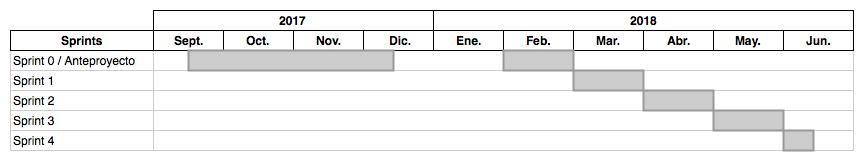
\includegraphics[width=1\textwidth]{/Planificacion_Temporal.png}
		\caption{Planificación Temporal}
		\label{fig:plantempo}
	\end{center}
\end{figure}

\clearpage

\section{Sprint 1: Diseño de una plataforma Web para la gestión de los usuarios}
Este primer Sprint está enfocado a diseñar e implementar una plataforma Web para la gestión de los usuarios de la aplicación de mensajería instantánea. De esta manera, tareas como las de añadir nuevos usuarios, consultar los existentes o modificarlos resulte mucho más sencillo, cómodo y práctico para los potenciales administradores de la plataforma que se pretende desarrollar, puesto que una de las principales premisas es su sencillez de uso, ofreciendo una interfaz más amigable que la que ofrece actualmente la base de datos de segunda generación de Firebase, Firestore. Además, se deberá crear una aplicación adicional en Java para cifrar las contraseñas de los nuevos administradores, de manera que nadie conozca la contraseña en claro del nuevo administrador.

\subsection{Planificación del Sprint}
Se han elegido las dos primeras historias de usuario para la consecución de este Sprint durante la reunión inicial (Tablas \ref{tab:historia1} y \ref{tab:historia2}).

\begin{table}[!htbp]
	\centering
	{\small
		\resizebox{15cm}{!} {
	\begin{tabular}{|l|l|}
		\hline
		\multicolumn{2}{|c|}{\cellcolor[HTML]{343434}{\color[HTML]{FFFFFF} \textbf{Historia de Usuario}}} \\
		\hline
		\multicolumn{2}{|c|}{\textbf{Sprint Asignado:} 3.} \\
		\hline
		\textbf{Número de Historia:} 5. & \textbf{Usuario/Rol:} Docente.\\
		\hline
		\multicolumn{2}{|l|}{\textbf{Nombre de la Historia:} Análisis del tono de los mensajes.} \\
		\hline
		\textbf{Prioridad:} Alta. & \textbf{Duración:} 4 horas.\\
		\hline
		\multicolumn{2}{|l|}{\textbf{Descripción:} Analizar el tono de los mensajes de los usuarios y mostrarlos al administrador del chat.} \\
		\hline
		\specialcell{\textbf{Tareas:} Creación e integración \\ de los servicios de IBM Bluemix. \\ Mostrar al administrador de chat \\ los tonos de cada mensaje y usuario.} & \textbf{Pruebas:} \\
		\hline
	\end{tabular}
}






%\begin{tabular}{| c | c | c | c | c | c |}
%	\hline
%	\multicolumn{6}{|c|}{\cellcolor[HTML]{000000}{\color[HTML]{FFFFFF} \textbf{Historia de Usuario}}} \\ 
%	\hline \multicolumn{6}{|c|}{\textbf{Sprint Asignado:} 1} \\
%	\hline \multicolumn{3}{|l|}{\textbf{Número de Historia:} 1} & \multicolumn{3}{l|}{\textbf{Usuario/Rol:} Administrador} \\
%	\hline \multicolumn{6}{|l|}{\textbf{Nombre de la Historia:} Gestión de usuarios de la aplicación móvil} \\
%	\hline \multicolumn{3}{|l|}{\textbf{Prioridad:} Alta} & \multicolumn{3}{l|}{\textbf{Duración:} 30 horas} \\
%	\hline \multicolumn{6}{|l|}{\textbf{Descripción:} Desarrollar una plataforma Web para facilitar la gestión de los usuarios de la aplicación móvil.} \\
%	\hline \multicolumn{6}{|l|}{\textbf{Tareas:}} \\
%	\hline
%\end{tabular}

% Local variables:
%   coding: utf-8
%   ispell-local-dictionary: "castellano8"
%   TeX-master: "main.tex"
% End:

	}
	\caption[Historia de Usuario 1]
	{Historia de Usuario 1}
	\label{tab:historia1}
\end{table}

\begin{table}[!htbp]
	\centering
	{\small
		\resizebox{15cm}{!} {
	\begin{tabular}{|l|l|}
		\hline
		\multicolumn{2}{|c|}{\cellcolor[HTML]{343434}{\color[HTML]{FFFFFF} \textbf{Historia de Usuario}}} \\
		\hline
		\multicolumn{2}{|c|}{\textbf{Sprint Asignado:} 2.} \\
		\hline
		\textbf{Número de Historia:} 3. & \textbf{Usuario/Rol:} Docente.\\
		\hline
		\multicolumn{2}{|l|}{\textbf{Nombre de la Historia:} Creación de chats grupales.} \\
		\hline
		\textbf{Prioridad:} Alta. & \textbf{Duración:} 10 horas.\\
		\hline
		\multicolumn{2}{|l|}{\textbf{Descripción:} Proporcionar al docente un método de crear un nuevo chat.} \\
		\hline
		\specialcell{\underline{\textbf{Tareas}} \\ Adecuación de la estructura de la base de datos. \\ Diseño de la actividad de creación de grupos.} & \specialcell{\underline{\textbf{Pruebas}} \\ Correcta creación del chat en la nueva colección. \\ Comprobar que se elige un nombre del chat válido. \\ Comprobar que se elige, al menos, una familia.} \\
		\hline
	\end{tabular}
}


	}
	\caption[Historia de Usuario 2]
	{Historia de Usuario 2}
	\label{tab:historia2}
\end{table}

%TODO: Extracto código algoritmo MD5
%TODO: LOPD
\subsection{Tareas del Sprint}
\subsubsection{Diseño inicial de la base de datos}
Firebase Firestore ofrece una base de datos no relacional, lo que significa que no existen relaciones ni tablas, como sí ocurre en las bases de datos relacionales. Por tanto, en este caso, se tienen colecciones de documentos que, a su vez, pueden tener colecciones de documentos anidadas. En consecuencia, se ha realizado un primer diseño en el que la base de datos tendrá tres colecciones: <<Usuarios>>, para los usuarios de las familias; <<UsuariosWeb>>, que albergará los administradores con acceso al sitio Web para la gestión de las familias y <<Docentes>>, que contendrá los datos de los docentes y potenciales administradores de los grupos de chat. Los campos que se guardarán de cada uno son los siguientes:

\begin{itemize}
	\item \textbf{Usuarios}.
		\begin{itemize}
			\item Nombre del Tutor Legal 1.
			\item Primer apellido del Tutor Legal 1.
			\item Segundo apellido del Tutor Legal 1.
			\item Teléfono del Tutor Legal 1.
			\item Correo electrónico del Tutor Legal 1.
			\item Nombre del Tutor Legal 2.
			\item Primer apellido del Tutor Legal 2.
			\item Segundo apellido del Tutor Legal 2.
			\item Teléfono del Tutor Legal 2.
			\item Correo electrónico del Tutor Legal 2.
		\end{itemize}
		
	\item \textbf{Docentes}.
		\begin{itemize}
			\item Nombre.
			\item Primer apellido.
			\item Segundo apellido.
			\item Correo electrónico.
			\item Teléfono.
		\end{itemize}
		
	\item \textbf{UsuariosWeb}.
		\begin{itemize}
			\item Correo electrónico.
			\item Contraseña.
		\end{itemize}
		
\end{itemize}

En cuanto a la gestión de contraseñas, no es necesario guardarlas en la base de datos, a excepción de las de los administradores con acceso al sitio Web puesto que, al hacer uso de la funcionalidad de Firebase \textit{Authentication}, éstas se guardan internamente en el proyecto y únicamente son conocidas por la herramienta, asignando además un identificador único de usuario a cada uno de los usuarios registrados.

\subsubsection{Implementación de la plataforma Web}
En el centro educativo existirá uno o varios administradores con acceso a la página Web que se encargarán de gestionar las familias de la base de datos para que, posteriormente, estas puedan acceder a la aplicación móvil. Por tanto, se contemplan las siguientes acciones: dar de alta, dar de baja, consultar y modificar. La plataforma Web debe proporcionar estas acciones de una manera sencilla, vistosa y \textit{responsive}. Para este propósito se ha decidido hacer uso de Bootstrap \cite{Bootstrap}, que proporciona un conjunto de herramientas para desarrollo con HTML, CSS y JavaScript. Del mismo modo, se ha incluido Firebase y las referencias a la base de datos de Firestore del proyecto. Por seguridad, el registro de un nuevo administrador en la base de datos se deberá llevar a cabo de manera manual, accediendo al proyecto de Firebase, donde se guardará un nuevo documento con el correo electrónico y la contraseña cifrada mediante el algoritmo SHA-1, que se obtendrá gracias a una aplicación desarrollada en la siguiente historia de usuario. Del mismo modo, se ha implementado un método para evitar que un usuario acceda a una página conocida dentro del servidor mediante el uso de \textit{Session Storage}. De esta manera, cuando el usuario accede correctamente con su correo y contraseña, el servidor genera y devuelve un número de sesión que se almacena en esta caché del navegador junto con el correo electrónico por lo que, si alguno de estos campos se encuentra sin definir en la caché en el momento de acceder a una página, se devuelve automáticamente al inicio de sesión (Figura \ref{fig:login_web}). Una vez se ha identificado en la página Web, el usuario accede a una página principal con cuatro botones y una barra de navegación superior desde donde puede realizar las cuatro acciones principales: dar de alta, dar de baja, consultar usuarios y modificar usuarios (Figura \ref{fig:index_web}). A continuación, se llevará a cabo una explicación de cada uno.

\begin{figure}[!h]
	\begin{center}
		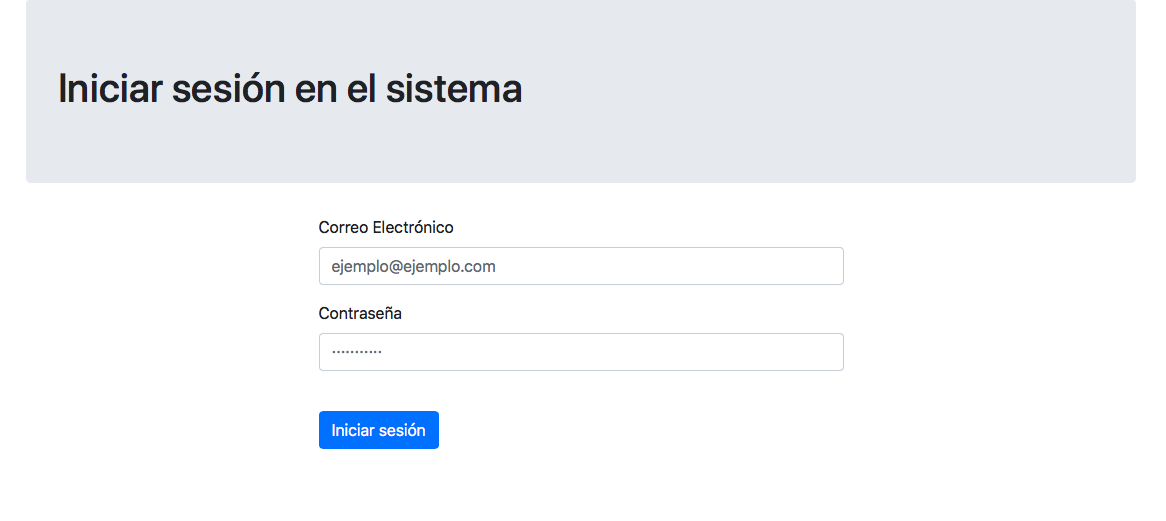
\includegraphics[width=0.9\textwidth]{/captura_login_web.png}
		\caption{Login de la Web}
		\label{fig:login_web}
	\end{center}
\end{figure}

\begin{figure}[!h]
	\begin{center}
		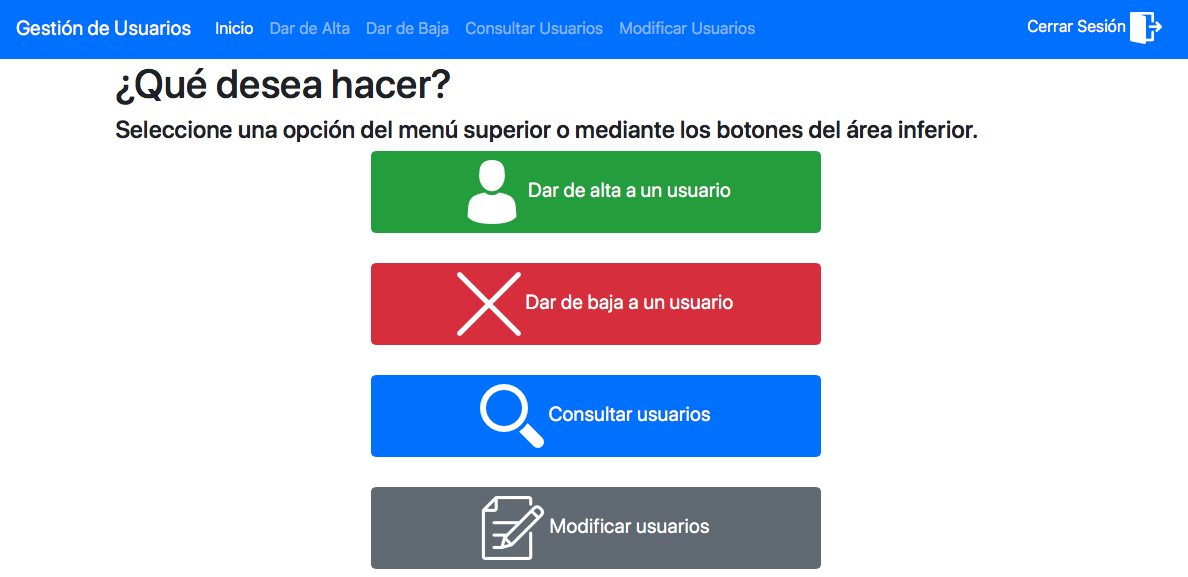
\includegraphics[width=0.9\textwidth]{/captura_index_web.png}
		\caption{Página Principal de la Web}
		\label{fig:index_web}
	\end{center}
\end{figure}

\newpage

\noindent \underline{Dar de Alta} \newline
En esta primera funcionalidad, el administrador tiene la opción de rellenar un formulario para registrar una nueva familia en la base de datos, en el que se pueden incluir los datos de un único tutor legal del alumno o, si lo hubiese, también los del segundo tutor. Los datos que se han especificado para cada tutor son: nombre, primer apellido, segundo apellido, número de teléfono y correo electrónico. Por último, para identificar a este usuario en la base de datos, se le asignará un identificador compuesto del primer apellido de ambos tutores o, en su defecto, del único tutor, concatenando un número al final. Es decir, si dos familias diferentes poseen los mismos apellidos, se añadirá un número al final de la composición de sus apellidos para el identificador, por lo que quedarán representadas de manera única en la base de datos. Por otra parte, además de disponer del formulario para introducir nuevos usuarios, el administrador también tiene la posibilidad de importar un archivo \acs{CSV} para realizar esta tarea de una manera más sencilla y automatizada. Este archivo debe tener un formato específico detallado en la primera línea del mismo y que consta, principalmente, de los mismos datos que en el formulario separados por comas y sin espacios entre ellos, separando cada familia por un salto de línea.

\noindent \underline{Dar de Baja} \newline
Al entrar en esta página, se dispone de una lista desplegable en la que se cargarán todas las familias registradas en la base de datos. Al seleccionar una de ellas, se cargarán automáticamente en una tabla los datos de la misma. Como medida adicional contra el borrado accidental, la página pedirá al usuario que confirme la acción de borrado solicitada antes de ser llevada a cabo.

\clearpage

\noindent \underline{Consultar Usuarios} \newline
De manera similar, se ha implementado una tabla para consultar los datos de los usuarios aunque, en este caso, se dispone de una herramienta básica de búsqueda en la que se puede filtrar por cada uno de los campos existentes en la base de datos. Si se pulsa el botón de buscar sin escribir nada en el filtro, la tabla se cargará con todos los registros existentes.

\noindent \underline{Modificar Usuarios} \newline
Esta funcionalidad se ha implementado mediante el uso de una lista desplegable que carga todas las familias de la base de datos y un formulario que inicialmente se muestra bloqueado para prevenir una modificación accidental de los datos. Al seleccionar uno de estos registros, su información se carga en dicho formulario y al hacer clic sobre el botón de modificar se habilitan los campos para la escritura. Cuando el administrador finalice la modificación de la información, deberá hacer clic de nuevo en un botón para terminar la modificación, siendo preguntado sobre si realmente desea llevarla a cabo. En caso positivo, se sobrescribirá la información de la familia seleccionada en la base de datos.

Como medida adicional de seguridad y en prevención de corrupción de datos, el sitio Web preguntará siempre al usuario si desea salir de la página en la que se encuentre, a excepción de la página de consulta de usuarios, puesto que no implica modificación alguna de datos.

\subsubsection{Desarrollo de una Aplicación Java de Cifrado}
Ya que un administrador será el responsable de registrar a nuevos administradores en la base de datos, deberá conocer el correo electrónico y la contraseña del nuevo administrador. Para mantener la contraseña lo más segura posible se ha decidido desarrollar una pequeña aplicación en Java cuya principal función sea la de cifrar la contraseña utilizando el cifrado SHA-1 de este nuevo administrador, que será la que se introduzca en la base de datos. Para ello, al iniciar la aplicación (Figura \ref{fig:cifrador}) se deberá escribir la contraseña en el campo correspondiente y hacer clic sobre el botón de cifrar para generar la cadena cifrada. Además, se dispone de un botón para copiarla en el portapapeles.

\begin{figure}[!h]
	\begin{center}
		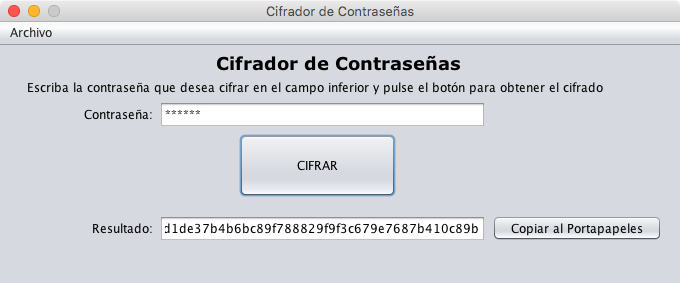
\includegraphics[width=0.8\textwidth]{/cifrador}
		\caption{Aplicación de Cifrado}
		\label{fig:cifrador}
	\end{center}
\end{figure}

\clearpage

\section{Sprint 2: Creación de la aplicación Android y creación de chats grupales}
Este Sprint está dedicado íntegramente a la aplicación para dispositivos móviles, con lo que esto conlleve en cuanto a las tareas de diseño y comunicación con la base de datos. De esta manera, los docentes (que serán los administradores de los chats) serán los únicos capaces de crear uno y las familias podrán ver todos a los que han sido añadidas. También cada uno de los usuarios de las familias será capaz de enviar mensajes que aparecerán en el grupo acompañados de su nombre junto con la fecha y hora de envío.

\subsection{Planificación del Sprint}
Para este segundo Sprint se han seleccionado las siguientes historias de usuario:

\begin{table}[!htbp]
	\centering
	{\small
		\resizebox{15cm}{!} {
	\begin{tabular}{|l|l|}
		\hline
		\multicolumn{2}{|c|}{\cellcolor[HTML]{343434}{\color[HTML]{FFFFFF} \textbf{Historia de Usuario}}} \\
		\hline
		\multicolumn{2}{|c|}{\textbf{Sprint Asignado:} 3.} \\
		\hline
		\textbf{Número de Historia:} 5. & \textbf{Usuario/Rol:} Docente.\\
		\hline
		\multicolumn{2}{|l|}{\textbf{Nombre de la Historia:} Análisis del tono de los mensajes.} \\
		\hline
		\textbf{Prioridad:} Alta. & \textbf{Duración:} 4 horas.\\
		\hline
		\multicolumn{2}{|l|}{\textbf{Descripción:} Analizar el tono de los mensajes de los usuarios y mostrarlos al administrador del chat.} \\
		\hline
		\specialcell{\textbf{Tareas:} Creación e integración \\ de los servicios de IBM Bluemix. \\ Mostrar al administrador de chat \\ los tonos de cada mensaje y usuario.} & \textbf{Pruebas:} \\
		\hline
	\end{tabular}
}






%\begin{tabular}{| c | c | c | c | c | c |}
%	\hline
%	\multicolumn{6}{|c|}{\cellcolor[HTML]{000000}{\color[HTML]{FFFFFF} \textbf{Historia de Usuario}}} \\ 
%	\hline \multicolumn{6}{|c|}{\textbf{Sprint Asignado:} 1} \\
%	\hline \multicolumn{3}{|l|}{\textbf{Número de Historia:} 1} & \multicolumn{3}{l|}{\textbf{Usuario/Rol:} Administrador} \\
%	\hline \multicolumn{6}{|l|}{\textbf{Nombre de la Historia:} Gestión de usuarios de la aplicación móvil} \\
%	\hline \multicolumn{3}{|l|}{\textbf{Prioridad:} Alta} & \multicolumn{3}{l|}{\textbf{Duración:} 30 horas} \\
%	\hline \multicolumn{6}{|l|}{\textbf{Descripción:} Desarrollar una plataforma Web para facilitar la gestión de los usuarios de la aplicación móvil.} \\
%	\hline \multicolumn{6}{|l|}{\textbf{Tareas:}} \\
%	\hline
%\end{tabular}

% Local variables:
%   coding: utf-8
%   ispell-local-dictionary: "castellano8"
%   TeX-master: "main.tex"
% End:

	}
	\caption[Historia de Usuario 3]
	{Historia de Usuario 3}
	\label{tab:historia3}
\end{table}

\begin{table}[!htbp]
	\centering
	{\small
		\resizebox{15cm}{!} {
	\begin{tabular}{|l|l|}
		\hline
		\multicolumn{2}{|c|}{\cellcolor[HTML]{343434}{\color[HTML]{FFFFFF} \textbf{Historia de Usuario}}} \\
		\hline
		\multicolumn{2}{|c|}{\textbf{Sprint Asignado:} 2.} \\
		\hline
		\textbf{Número de Historia:} 3. & \textbf{Usuario/Rol:} Docente.\\
		\hline
		\multicolumn{2}{|l|}{\textbf{Nombre de la Historia:} Creación de chats grupales.} \\
		\hline
		\textbf{Prioridad:} Alta. & \textbf{Duración:} 10 horas.\\
		\hline
		\multicolumn{2}{|l|}{\textbf{Descripción:} Proporcionar al docente un método de crear un nuevo chat.} \\
		\hline
		\specialcell{\underline{\textbf{Tareas}} \\ Adecuación de la estructura de la base de datos. \\ Diseño de la actividad de creación de grupos.} & \specialcell{\underline{\textbf{Pruebas}} \\ Correcta creación del chat en la nueva colección. \\ Comprobar que se elige un nombre del chat válido. \\ Comprobar que se elige, al menos, una familia.} \\
		\hline
	\end{tabular}
}


	}
	\caption[Historia de Usuario 4]
	{Historia de Usuario 4}
	\label{tab:historia4}
\end{table}

\begin{table}[!htbp]
	\centering
	{\small
		\resizebox{15cm}{!} {
	\begin{tabular}{|l|l|}
		\hline
		\multicolumn{2}{|c|}{\cellcolor[HTML]{343434}{\color[HTML]{FFFFFF} \textbf{Historia de Usuario}}} \\
		\hline
		\multicolumn{2}{|c|}{\textbf{Sprint Asignado:} 2.} \\
		\hline
		\textbf{Número de Historia:} 5. & \textbf{Usuario/Rol:} Docente, Familia.\\
		\hline
		\multicolumn{2}{|l|}{\textbf{Nombre de la Historia:} Envío y recepción de mensajes de un determinado chat.} \\
		\hline
		\textbf{Prioridad:} Alta. & \textbf{Duración:} 8 horas.\\
		\hline
		\multicolumn{2}{|l|}{\textbf{Descripción:} Añadir capacidad de poder enviar y leer mensajes de los chats de los que se es miembro.} \\
		\hline
		\specialcell{\underline{\textbf{Tareas}} \\ Diseño de la actividad principal. \\ Diseño de la actividad de grupo.} & \specialcell{\underline{\textbf{Pruebas}} \\ Únicamente se muestran chats de los que se es miembro. \\ Carga de chats al iniciar la aplicación. \\ Carga de mensajes al abrir el chat. \\ Desplazamiento al último mensaje cuando se recibe uno nuevo.} \\
		\hline
	\end{tabular}
}

	}
	\caption[Historia de Usuario 5]
	{Historia de Usuario 5}
	\label{tab:historia5}
\end{table}

\newpage

\subsection{Tareas del Sprint}
\subsubsection{Diseño de la actividad de acceso}
Esta tarea requiere de la integración previa de Firebase con la aplicación Android, por lo que se han seguido los pasos necesarios indicados por la propia herramienta gracias a su integración con Android Studio para que dicha aplicación pueda comunicarse con los servicios que ofrece la plataforma de Google. Una vez hecho esto, se procede a diseñar la actividad de acceso desde la que los usuarios podrán identificarse en el sistema antes de poder visualizar o enviar mensajes al mismo. Desde un primer momento se ha separado la identificación de los usuarios mediante un \textit{login} <<normal>> y otro específico para docentes, que se muestra mediante un botón independiente, como se puede ver en la Figura \ref{fig:login1}.

\begin{figure}[!h]
	\begin{center}
		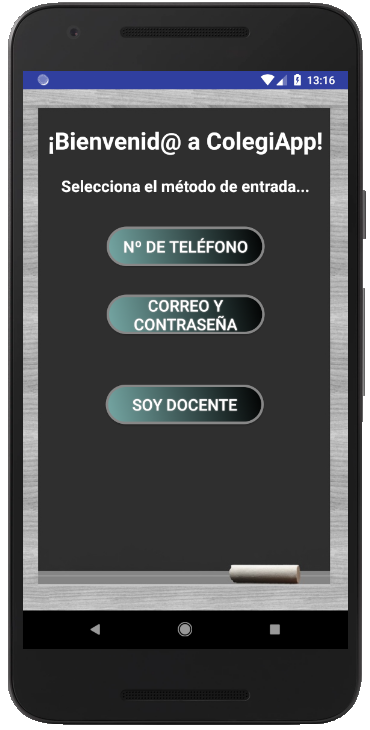
\includegraphics[width=0.31\textwidth]{/capturas_app/login1.png}
		\caption{Actividad inicial}
		\label{fig:login1}
	\end{center}
\end{figure}

\newpage

En el caso de seleccionar el número de teléfono como método de entrada, la aplicación preguntará por un número de teléfono (Figura \ref{fig:logintfno}) al usuario, comprobará su existencia en la base de datos y, si el resultado es positivo, se le mandará un mensaje vía \acs{SMS} con un código que se debe introducir antes de 60 segundos para que el sistema pueda registrar al usuario mediante Firebase \textit{Authentication}. En caso de no existir ese número en la base de datos, se alertará con un mensaje, no pudiendo acceder a la aplicación

\begin{figure}[!h]
	\begin{center}
		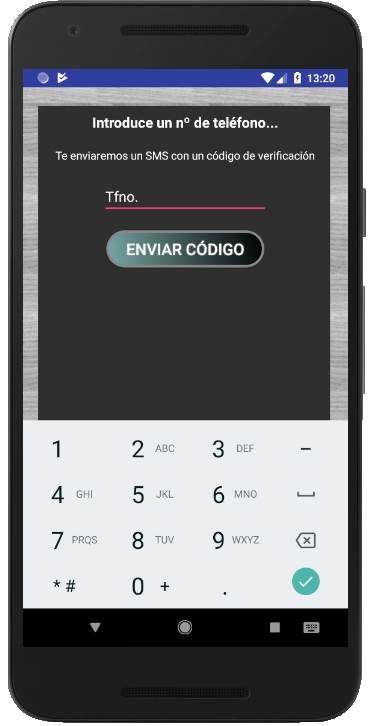
\includegraphics[width=0.35\textwidth]{/capturas_app/logintfno.png}
		\caption{Actividad \textit{login} con teléfono}
		\label{fig:logintfno}
	\end{center}
\end{figure}

Por el contrario, si el usuario decide acceder mediante un correo electrónico y una contraseña, este deberá introducir ambos campos (Figura \ref{fig:logincorreo}) y, de nuevo, se realizará una primera comprobación de su existencia en la base de datos. En caso de que sea la primera vez que se accede a la aplicación no dispondrá de ninguna contraseña asignada, por lo que la contraseña que se introduzca por primera vez será la que el sistema utilizará para su identificación en futuras ocasiones, pudiendo ser cambiada.

\clearpage

Si el usuario no recuerda su contraseña o decide cambiarla, podrá hacerlo mediante la función <<¿Has olvidado tu contraseña?>>, en la que deberá introducir su correo y, acto seguido, el sistema enviará un mensaje de recuperación a la dirección de correo indicada siempre que se encuentre registrada en la base de datos. Dicho mensaje contendrá una dirección Web a la que el usuario debe entrar para introducir su nueva contraseña (Figura \ref{fig:cambiopass}). Una vez finalizado el proceso, podrá acceder al sistema con su nueva clave.

\begin{figure}[!h]
	\centering
	\begin{minipage}{.5\textwidth}
		\centering
		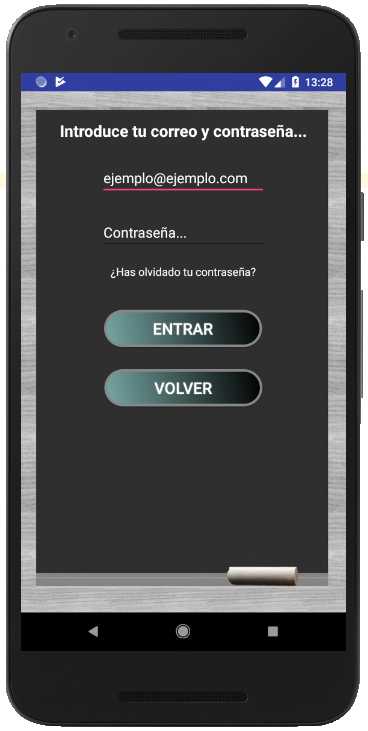
\includegraphics[width=0.7\textwidth]{/capturas_app/logincorreo.png}
		\caption{Actividad \textit{login} con correo y contraseña}
		\label{fig:logincorreo}
	\end{minipage}%
	\begin{minipage}{.5\textwidth}
		\centering
		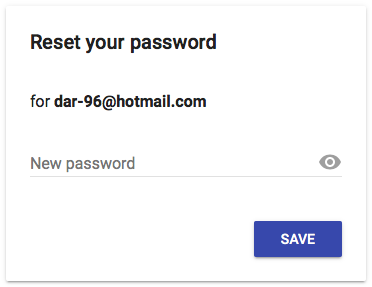
\includegraphics[width=0.7\textwidth]{/capturas_app/cambiopass.png}
		\caption{Cambio de contraseña}
		\label{fig:cambiopass}
	\end{minipage}
\end{figure}

\clearpage

Por otra parte, si quien quiere acceder a la aplicación es un docente, este deberá seleccionar la opción <<Soy Docente>>, en cuyo caso se preguntará si quiere autenticarse mediante número de teléfono o mediante correo y contraseña (Figura \ref{fig:logindocente}), siendo los siguientes pasos iguales a los descritos anteriormente para un usuario perteneciente a una familia.

\begin{figure}[!h]
	\begin{center}
		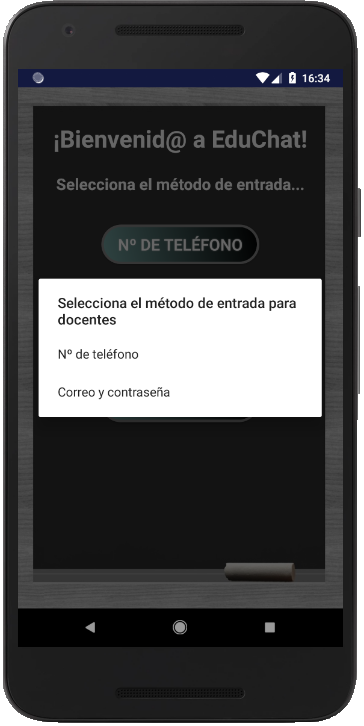
\includegraphics[width=0.35\textwidth]{/capturas_app/logindocente.png}
		\caption{Autenticación del docente}
		\label{fig:logindocente}
	\end{center}
\end{figure}

\subsubsection{Adecuación de la base de datos}
A la hora de guardar los grupos de chat, se debe crear una nueva colección en la base de datos con todos los datos de los mismos a la que se le ha asignado el nombre de <<ChatsGrupales>>. En esta colección se encuentra un documento <<Control>> con un campo <<Contador>>, que se trata de un número entero usado para otorgar un identificador único a cada una de las salas de chat en la base de datos y que se irá incrementando a medida que se vayan creando nuevas. Cada uno de dichos documentos contendrá elementos como un objeto de tipo <<Administrador>>, que representará al docente creador del grupo con todos sus datos; su identificador en la base de datos y el nombre que el docente haya asignado a dicho grupo. Además, contendrá colecciones adicionales como <<Familias>> y <<Mensajes>>. La primera incluye los documentos de la colección <<Usuarios>> que el administrador haya incluido en el grupo, es decir, las familias participantes. Por su parte, la colección <<Mensajes>>, incluye documentos con los mensajes que cada integrante ha enviado al chat, conteniendo cada uno información del remitente, así como la fecha y hora de envío.

\subsubsection{Diseño de la actividad de creación de chats}
Esta funcionalidad está disponible únicamente para los docentes identificados en la aplicación, puesto que son los únicos usuarios con capacidad para iniciar nuevos chats. Una vez que el docente se ha identificado en el sistema y ha accedido a la actividad principal, podrá crear un nuevo chat mediante la opción <<Crear nuevo chat>> situada en el menú principal de la aplicación, que se encuentra en la esquina superior derecha de la pantalla. Al seleccionar esta opción, se mostrará una nueva actividad en la que se podrá introducir el nombre del grupo y los integrantes del mismo (Figura \ref{fig:creargrupo}) mediante una lista en la que se mostrarán todas las familias que se encuentren en ese momento en la colección <<Usuarios>> de la base de datos. Para finalizar su creación, se debe pulsar el botón <<Crear Chat>>, en cuyo caso la aplicación preguntará al docente si realmente desea crear ese grupo y se le devolverá a la actividad principal, donde se muestran los grupos de los que el usuario es miembro.

\begin{figure}[!h]
	\begin{center}
		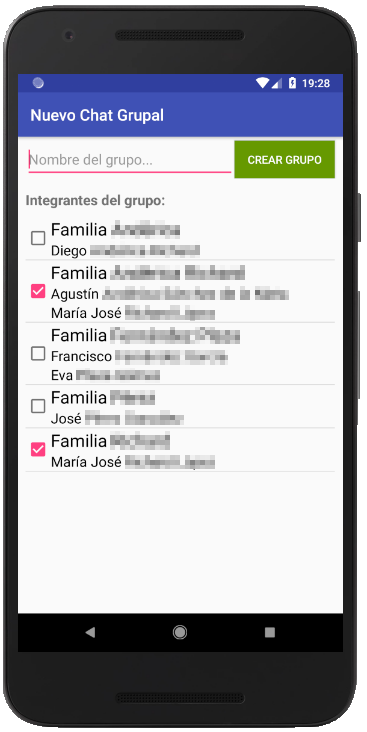
\includegraphics[width=0.35\textwidth]{/capturas_app/creargrupo.png}
		\caption{Actividad Crear Chat}
		\label{fig:creargrupo}
	\end{center}
\end{figure}

\newpage

\subsubsection{Diseño de la actividad principal}
Esta actividad será la primera que el usuario visualice nada más entrar a la aplicación y, por tanto, su principal función reside en mostrar una lista con los chats de los que sea miembro. Dicha actividad se conectará a la base de datos y buscará en la colección <<Familias>> de cada uno de los documentos de chats de la colección <<ChatsGrupales>> para comprobar su pertenencia a los mismos. Durante este rápido proceso, puesto que en las pruebas nunca ha durado más de 2 segundos, se mostrará al usuario un diálogo de carga que, una vez completada la tarea de búsqueda, mostrará la lista ya cargada con todos los grupos a los que se tiene acceso y en los que el usuario podrá pulsar para acceder a ellos, abriendo la actividad responsable de mostrar los mensajes.

\subsubsection{Diseño de la actividad de chat}
Por último, la principal función de la actividad de chat es la de mostrar todos los mensajes que se han ido mandando desde su creación. En este caso, a diferencia de la actividad principal, donde se ha implementado una \textit{ListView}, en la actividad de grupo se ha utilizado una \textit{RecyclerView} (Figura \ref{fig:listview}) pensando en la eficiencia de la aplicación. Una \textit{RecyclerView} es una lista en la que se <<reciclan>> las filas de esta cuando el usuario se desplaza hacia arriba o hacia abajo y no se están mostrando. Por tanto, el rendimiento aumenta al tener muchas filas o, en este caso, mensajes en un grupo. El siguiente ejemplo representa un ejemplo de un posible grupo (Figura \ref{fig:ejemplogrupo}) 

\begin{figure}[!h]
	\centering
	\begin{minipage}{.5\textwidth}
		\centering
		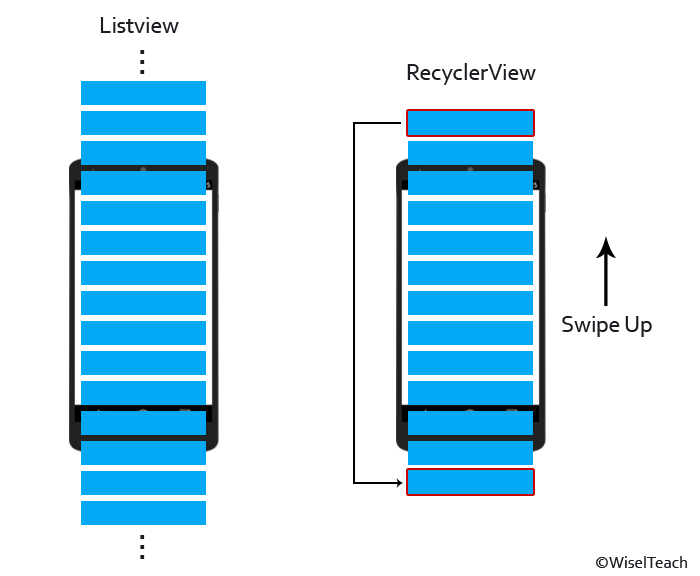
\includegraphics[width=1\linewidth]{listview.png}
		\caption{\textit{ListView} vs \textit{RecyclerView}}
		\label{fig:listview}{\url{https://goo.gl/2DreNc} (\url{www.medium.com})}
	\end{minipage}%
	\begin{minipage}{.5\textwidth}
		\centering
		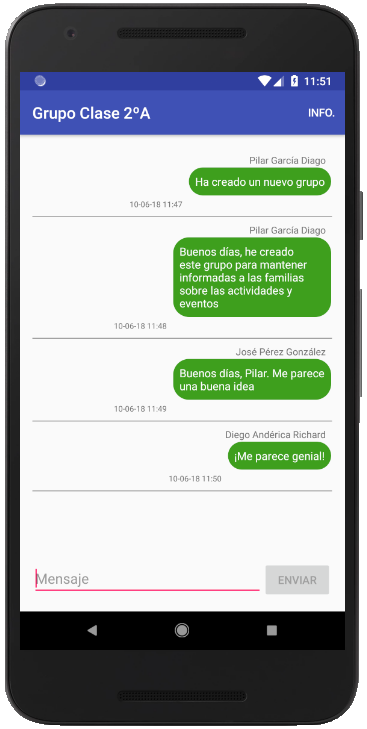
\includegraphics[width=0.65\linewidth]{/capturas_app/ejemplogrupo.png}
		\caption{Ejemplo de un grupo}
		\label{fig:ejemplogrupo}
	\end{minipage}
\end{figure}

\clearpage

\section{Sprint 3: Integración con los servicios Watson de IBM}
Este Sprint está principalmente enfocado a la creación, integración y manejo de resultados de los servicios de Watson que ofrece IBM mediante la plataforma IBM Bluemix. Gracias a esto, los docentes podrán obtener valores acerca del tono de conversación usado por los usuarios, divididos por mensajes y por grupo. En el primer caso, se visualizará mediante colores en los mensajes, mientras que en el segundo se mostrará mediante un porcentaje junto al nombre de cada usuario en la información del chat. Todo esto únicamente será visible para los administradores del chat.

\subsection{Planificación del Sprint}
En este tercer Sprint se ha seleccionado la siguiente historia de usuario para conformar el \textit{Sprint Backlog}:

\begin{table}[hp]
	\centering
	{\small
		\resizebox{15cm}{!} {
	\begin{tabular}{|l|l|}
		\hline
		\multicolumn{2}{|c|}{\cellcolor[HTML]{343434}{\color[HTML]{FFFFFF} \textbf{Historia de Usuario}}} \\
		\hline
		\multicolumn{2}{|c|}{\textbf{Sprint Asignado:} 3.} \\
		\hline
		\textbf{Número de Historia:} 5. & \textbf{Usuario/Rol:} Docente.\\
		\hline
		\multicolumn{2}{|l|}{\textbf{Nombre de la Historia:} Análisis del tono de los mensajes.} \\
		\hline
		\textbf{Prioridad:} Alta. & \textbf{Duración:} 4 horas.\\
		\hline
		\multicolumn{2}{|l|}{\textbf{Descripción:} Analizar el tono de los mensajes de los usuarios y mostrarlos al administrador del chat.} \\
		\hline
		\specialcell{\textbf{Tareas:} Creación e integración \\ de los servicios de IBM Bluemix. \\ Mostrar al administrador de chat \\ los tonos de cada mensaje y usuario.} & \textbf{Pruebas:} \\
		\hline
	\end{tabular}
}






%\begin{tabular}{| c | c | c | c | c | c |}
%	\hline
%	\multicolumn{6}{|c|}{\cellcolor[HTML]{000000}{\color[HTML]{FFFFFF} \textbf{Historia de Usuario}}} \\ 
%	\hline \multicolumn{6}{|c|}{\textbf{Sprint Asignado:} 1} \\
%	\hline \multicolumn{3}{|l|}{\textbf{Número de Historia:} 1} & \multicolumn{3}{l|}{\textbf{Usuario/Rol:} Administrador} \\
%	\hline \multicolumn{6}{|l|}{\textbf{Nombre de la Historia:} Gestión de usuarios de la aplicación móvil} \\
%	\hline \multicolumn{3}{|l|}{\textbf{Prioridad:} Alta} & \multicolumn{3}{l|}{\textbf{Duración:} 30 horas} \\
%	\hline \multicolumn{6}{|l|}{\textbf{Descripción:} Desarrollar una plataforma Web para facilitar la gestión de los usuarios de la aplicación móvil.} \\
%	\hline \multicolumn{6}{|l|}{\textbf{Tareas:}} \\
%	\hline
%\end{tabular}

% Local variables:
%   coding: utf-8
%   ispell-local-dictionary: "castellano8"
%   TeX-master: "main.tex"
% End:

	}
	\caption[Historia de Usuario 6]
	{Historia de Usuario 6}
	\label{tab:historia6}
\end{table}

\subsection{Tareas del Sprint}
\subsubsection{Creación e integración de los servicios de IBM Bluemix}
En primer lugar, se deben crear los servicios en la nube de IBM. Una vez hecho esto, se pueden integrar los paquetes necesarios en el proyecto. Se ha observado que el módulo de Watson \textit{Tone Analyzer} únicamente proporciona actualmente soporte para los idiomas inglés y francés a la hora de realizar consultas directamente, por lo que se ha optado por traducir previamente el texto a analizar. Esta traducción se realiza mediante el servicio \textit{Language Translator}, que también se encuentra disponible en la misma plataforma Watson, llevando a cabo todas las consultas mediante peticiones HTML en ambos servicios. De esta manera, el texto que introduzcan los usuarios de las familias sufrirá una traducción al idioma inglés y, posteriormente, un análisis del tono, que será recogido en la puntuación de cada uno de los mensajes que se manden, así como para computar el porcentaje total del usuario dentro de un chat que, en cierto modo, reflejará el estado de ánimo de este. Estas puntuaciones oscilarán entre valores que van del 0\% al 100\%, siendo el 0 el valor menos deseable y el 100 el valor óptimo o más deseable.

\clearpage

El servicio \textit{Tone Analyzer} puede analizar una única oración o un conjunto de ellas. Por tanto, en caso de que un usuario envíe un texto en el que se incluyan varias oraciones, se analizarán por separado y se calculará el resultado final teniendo en cuenta los resultados individuales. Asimismo, puede devolver diferentes tonos, cada uno con una <<puntuación>> que variará entre 0.5 y 1. Este valor no comienza en 0 puesto que IBM ha determinado que hay una mayor probabilidad de que se perciba el tono devuelto a partir de 0.5; por debajo de esa puntuación no se reconoce tono alguno, pues podría ser demasiado ambiguo o no determinante. \textit{Tone Analyzer} distingue entre tonos emocionales y tonos del lenguaje, siendo los siguientes los diferentes tonos que puede devolver este servicio \cite{IBM2018}:

\begin{itemize}
	\item \textbf{Enfado (tono emocional)}. El enfado se debe a la injusticia, conflicto, humillación, negligencia o traición. Si este tono es <<activo>>, la persona ataca al objetivo verbal o físicamente. Por el contrario, si es <<pasivo>>, la persona tendrá mal humor y sentirá tensión y hostilidad.
	\item \textbf{Miedo (tono emocional)}. El miedo es una respuesta al peligro inminente. Es un mecanismo de supervivencia que se desencadena como reacción a algún estímulo negativo. El miedo puede ser producto de la precaución o una fobia extrema.
	\item \textbf{Felicidad/alegría (tono emocional)}. Tiene matices de disfrute, satisfacción y placer. La alegría trae una sensación de bienestar, paz interior, amor, seguridad y satisfacción.
	\item \textbf{Tristeza (tono emocional)}. La tristeza indica una sensación de pérdida y desventaja. Cuando una persona está callada, menos enérgica y retraída, se puede deducir que siente tristeza.
	\item \textbf{Analítico (tono del lenguaje)}. Un tono analítico indica el razonamiento y la actitud analítica de una persona sobre las cosas. Una persona analítica puede ser percibida como intelectual, racional, sistemática o sin emociones.
	\item \textbf{Seguridad (tono del lenguaje)}. Un tono de confianza o seguridad indica el grado de certeza de una persona. Una persona segura de sí misma puede ser percibida como segura, coleccionada, optimista o egoísta.
	\item \textbf{Tentativo (tono del lenguaje)}. Un tono tentativo indica el grado de inhibición de una persona. Una persona tentativa puede ser percibida como cuestionable, dudosa o discutible.
\end{itemize}

\clearpage

Por tanto, en cuanto a tonos relacionados con las emociones, se han considerado como negativos el enfado, el miedo y la tristeza, quedando la felicidad como único tono positivo o deseable dentro de una conversación de chat. Por otra parte, en cuanto a los tonos del lenguaje, se han considerado como tonos de <<refuerzo>> para los tonos emocionales. Es decir, si se ha detectado tristeza con tono de seguridad, agravará la puntuación del mensaje y, por consiguiente, la puntuación total del usuario en el chat. Lo mismo ocurriría con la combinación de enfado y analítico aunque, en este caso, el tono analítico tendría menos peso que el de seguridad ya que se han asignado diferentes pesos por defecto a cada uno de los tonos. Puesto que se ha considerado el enfado como el menos deseable, se le ha asignado un 33.333\%; a la tristeza, un 29.166\%; al miedo, un 29.166\%; y a la alegría, un 8.333\%. De esta manera, los tonos considerados como <<negativos>> bajarán más rápidamente la puntuación del usuario y sus mensajes, siendo más difícil aumentarla. En cuanto a los pesos en tanto por uno de los tonos del lenguaje se han determinado los siguientes valores: para el analítico, un 0.666; para el de seguridad, un 0.166; y para el tentativo, un 0.166. Para estos últimos tonos también se dispone de otro valor para especificar el peso máximo que se puede añadir o sustraer a los tonos emocionales siendo, por defecto, de un 10\%. Es decir, los tonos del lenguaje podrán sustraer o añadir hasta un máximo de 10 unidades a la puntuación obtenida de los tonos emocionales. Todos estos valores se especifican por defecto al crear un chat y son independientes entre los diferentes documentos de chat de la base de datos, siendo posible su modificación, asignando diferentes pesos en cada uno de los chats.

Puesto que se dispone de una puntuación por mensaje y por usuario en el chat, se debe proporcionar una manera de visualizar estos valores al administrador del mismo. Para ello, se ha decidido mostrar mediante un código de colores la puntuación de cada mensaje. De esta manera, el administrador del chat podrá ver los colores rojo, naranja, amarillo o verde, en función de la puntuación de cada mensaje (Figura ). Por otro lado, la puntuación de cada usuario integrante se podrá consultar en forma de porcentaje (siendo el 0\% el peor valor y el 100\% el mejor o más deseable) mediante una actividad que se desarrollará en el siguiente Sprint cuya principal función será la de informar acerca de los datos del chat como el nombre (también se podrá modificar) y una lista de sus integrantes.

Debido a la inclusión de los tonos por mensaje y por usuario en la base de datos se ha tenido que llevar a cabo una ligera modificación de esta en lo que a la colección <<ChatsGrupales>> respecta. En cada uno de los chats se ha agregado un objeto <<PonderaciónTonos>>, que recogerá los pesos de cada uno de los tonos para cada chat y una colección adicional <<Tonos>>, que contendrá los tonos de cada uno de los integrantes del chat.

\clearpage

%TODO: Insertar imágenes de chat con colores y actividad de información de grupo.

\section{Sprint 4: Integración con Google Calendar y otras mejoras}
Este último Sprint se ha dedicado a añadir funcionalidades a las ya existentes de cara a completar la aplicación final, puesto que la principal función de comunicación ya ha sido implementada en Sprints anteriores. Algunas de estas mejoras son la integración con Google Calendar o la posibilidad de editar el perfil de un usuario de la aplicación.

\subsection{Planificación del Sprint}
En este Sprint se han seleccionado las siguientes historias de usuario:

\begin{table}[hp]
	\centering
	{\small
		\resizebox{15cm}{!} {
	\begin{tabular}{|l|l|}
		\hline
		\multicolumn{2}{|c|}{\cellcolor[HTML]{343434}{\color[HTML]{FFFFFF} \textbf{Historia de Usuario}}} \\
		\hline
		\multicolumn{2}{|c|}{\textbf{Sprint Asignado:} 3.} \\
		\hline
		\textbf{Número de Historia:} 5. & \textbf{Usuario/Rol:} Docente.\\
		\hline
		\multicolumn{2}{|l|}{\textbf{Nombre de la Historia:} Análisis del tono de los mensajes.} \\
		\hline
		\textbf{Prioridad:} Alta. & \textbf{Duración:} 4 horas.\\
		\hline
		\multicolumn{2}{|l|}{\textbf{Descripción:} Analizar el tono de los mensajes de los usuarios y mostrarlos al administrador del chat.} \\
		\hline
		\specialcell{\textbf{Tareas:} Creación e integración \\ de los servicios de IBM Bluemix. \\ Mostrar al administrador de chat \\ los tonos de cada mensaje y usuario.} & \textbf{Pruebas:} \\
		\hline
	\end{tabular}
}






%\begin{tabular}{| c | c | c | c | c | c |}
%	\hline
%	\multicolumn{6}{|c|}{\cellcolor[HTML]{000000}{\color[HTML]{FFFFFF} \textbf{Historia de Usuario}}} \\ 
%	\hline \multicolumn{6}{|c|}{\textbf{Sprint Asignado:} 1} \\
%	\hline \multicolumn{3}{|l|}{\textbf{Número de Historia:} 1} & \multicolumn{3}{l|}{\textbf{Usuario/Rol:} Administrador} \\
%	\hline \multicolumn{6}{|l|}{\textbf{Nombre de la Historia:} Gestión de usuarios de la aplicación móvil} \\
%	\hline \multicolumn{3}{|l|}{\textbf{Prioridad:} Alta} & \multicolumn{3}{l|}{\textbf{Duración:} 30 horas} \\
%	\hline \multicolumn{6}{|l|}{\textbf{Descripción:} Desarrollar una plataforma Web para facilitar la gestión de los usuarios de la aplicación móvil.} \\
%	\hline \multicolumn{6}{|l|}{\textbf{Tareas:}} \\
%	\hline
%\end{tabular}

% Local variables:
%   coding: utf-8
%   ispell-local-dictionary: "castellano8"
%   TeX-master: "main.tex"
% End:

	}
	\caption[Historia de Usuario 7]
	{Historia de Usuario 7}
	\label{tab:historia7}
\end{table}

\begin{table}[hp]
	\centering
	{\small
		\resizebox{15cm}{!} {
	\begin{tabular}{|l|l|}
		\hline
		\multicolumn{2}{|c|}{\cellcolor[HTML]{343434}{\color[HTML]{FFFFFF} \textbf{Historia de Usuario}}} \\
		\hline
		\multicolumn{2}{|c|}{\textbf{Sprint Asignado:} 2.} \\
		\hline
		\textbf{Número de Historia:} 3. & \textbf{Usuario/Rol:} Docente.\\
		\hline
		\multicolumn{2}{|l|}{\textbf{Nombre de la Historia:} Creación de chats grupales.} \\
		\hline
		\textbf{Prioridad:} Alta. & \textbf{Duración:} 10 horas.\\
		\hline
		\multicolumn{2}{|l|}{\textbf{Descripción:} Proporcionar al docente un método de crear un nuevo chat.} \\
		\hline
		\specialcell{\underline{\textbf{Tareas}} \\ Adecuación de la estructura de la base de datos. \\ Diseño de la actividad de creación de grupos.} & \specialcell{\underline{\textbf{Pruebas}} \\ Correcta creación del chat en la nueva colección. \\ Comprobar que se elige un nombre del chat válido. \\ Comprobar que se elige, al menos, una familia.} \\
		\hline
	\end{tabular}
}


	}
	\caption[Historia de Usuario 8]
	{Historia de Usuario 8}
	\label{tab:historia8}
\end{table}

\begin{table}[hp]
	\centering
	{\small
		\resizebox{15cm}{!} {
	\begin{tabular}{|l|l|}
		\hline
		\multicolumn{2}{|c|}{\cellcolor[HTML]{343434}{\color[HTML]{FFFFFF} \textbf{Historia de Usuario}}} \\
		\hline
		\multicolumn{2}{|c|}{\textbf{Sprint Asignado:} 2.} \\
		\hline
		\textbf{Número de Historia:} 5. & \textbf{Usuario/Rol:} Docente, Familia.\\
		\hline
		\multicolumn{2}{|l|}{\textbf{Nombre de la Historia:} Envío y recepción de mensajes de un determinado chat.} \\
		\hline
		\textbf{Prioridad:} Alta. & \textbf{Duración:} 8 horas.\\
		\hline
		\multicolumn{2}{|l|}{\textbf{Descripción:} Añadir capacidad de poder enviar y leer mensajes de los chats de los que se es miembro.} \\
		\hline
		\specialcell{\underline{\textbf{Tareas}} \\ Diseño de la actividad principal. \\ Diseño de la actividad de grupo.} & \specialcell{\underline{\textbf{Pruebas}} \\ Únicamente se muestran chats de los que se es miembro. \\ Carga de chats al iniciar la aplicación. \\ Carga de mensajes al abrir el chat. \\ Desplazamiento al último mensaje cuando se recibe uno nuevo.} \\
		\hline
	\end{tabular}
}

	}
	\caption[Historia de Usuario 9]
	{Historia de Usuario 9}
	\label{tab:historia9}
\end{table}

\begin{table}[!htbp]
	\centering
	{\small
		\resizebox{15cm}{!} {
	\begin{tabular}{|l|l|}
		\hline
		\multicolumn{2}{|c|}{\cellcolor[HTML]{343434}{\color[HTML]{FFFFFF} \textbf{Historia de Usuario}}} \\
		\hline
		\multicolumn{2}{|c|}{\textbf{Sprint Asignado:} 4.} \\
		\hline
		\textbf{Número de Historia:} 10. & \textbf{Usuario/Rol:} Administrador.\\
		\hline
		\multicolumn{2}{|l|}{\textbf{Nombre de la Historia:} Visualización de la información de los integrantes.} \\
		\hline
		\textbf{Prioridad:} Moderada. & \textbf{Duración:} 1 hora.\\
		\hline
		\multicolumn{2}{|l|}{\textbf{Descripción:} Capacidad para ver la información de los integrantes del chat.} \\
		\hline
		\specialcell{\underline{\textbf{Tareas}} \\ Lanzar actividad de perfil desde la de \\ información de grupo.} & \specialcell{\underline{\textbf{Pruebas}} \\ Comprobar que se muestran los datos de \\ la familia seleccionada.} \\
		\hline
	\end{tabular}
}

	}
	\caption[Historia de Usuario 10]
	{Historia de Usuario 10}
	\label{tab:historia10}
\end{table}

\subsection{Tareas del Sprint}
%TODO: Poner imagen correo integrantes.
\subsubsection{Integración con Google Calendar}
Para esta funcionalidad se ha añadido un botón (+) (Figura \ref{fig:crearevento}) que lanzará la aplicación de Google Calendar y permitirá al administrador del chat crear un nuevo evento al que serán añadidos los correos electrónicos de los integrantes como <<invitados>> del mismo. Este botón únicamente será visible para los administradores del chat, no mostrándose al resto de integrantes.

\begin{figure}[!h]
	\begin{center}
		
\includegraphics[width=0.4\textwidth]{/capturas_app/calendario.png}
		\caption{Botón para crear evento}
		\label{fig:crearevento}
	\end{center}
\end{figure}

\subsubsection{Creación y modificación del perfil}
Esta funcionalidad está disponible para todos los usuarios desde la actividad principal mediante una opción en el menú (Figura \ref{fig:menuppal}). Esta opción lanzará una nueva actividad desde la que se podrá editar la imagen de perfil, pudiendo seleccionar una desde la galería o retirarla para establecer la imagen por defecto. Del mismo modo, se muestra al usuario sus datos personales que se encuentran en la base de datos.

%TODO: Poner captura info perfil

\begin{figure}[!h]
	\begin{center}
		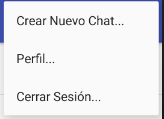
\includegraphics[width=0.3\textwidth]{/capturas_app/menuppal.png}
		\caption{Menú principal}
		\label{fig:menuppal}
	\end{center}
\end{figure}

\subsubsection{Eliminar y cambiar nombre de un chat}
Mediante estas opciones se facilita la tarea de gestión de los chats a los administradores de los mismos. Para eliminar un chat bastará con dejarlo pulsado en la lista de la actividad principal mostrándose un cuadro de diálogo confirmando la eliminación (Figura \ref{fig:borrarchat}). Por otra parte, si lo que se desea es cambiar el nombre de un chat, primero se deberá entrar en el mismo y pulsar en el botón <<Info.>>, que se encuentra en la parte superior derecha. Inmediatamente se accederá a la actividad de información de grupo que se ha desarrollado para, además de cambiar el nombre, poder observar qué familias lo conforman mediante una lista. Además, al lado de cada usuario se puede consultar un número en forma de porcentaje que representa el tono general que ha empleado en el grupo, siendo el 100\% el mejor valor posible, como se ha detallado en el Sprint anterior.

\begin{figure}[!h]
	\begin{center}
		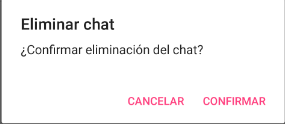
\includegraphics[width=0.4\textwidth]{/capturas_app/borrarchat.png}
		\caption{Diálogo para borrar un chat}
		\label{fig:borrarchat}
	\end{center}
\end{figure}

%TODO: Insertar captura info familia.
\subsubsection{Visualizar información de los integrantes}
Para el administrador de un chat, probablemente sea de utilidad proporcionar la información de cada uno de los integrantes del chat. Por este motivo se ha decidido implementar esta funcionalidad, que será accesible desde la actividad de información de chat, pulsando sobre alguno de los integrantes. De esta manera, se lanzará la actividad de perfil desde la que se podrá acceder a la información de la familia, así como a la foto de perfil, si estuviera definida.








